\documentclass[11pt]{article}
\usepackage[margin=1in]{geometry}
\usepackage{amsmath}
\usepackage[version=4]{mhchem}
\usepackage[T1]{fontenc}
\usepackage{lmodern}
\usepackage[authoryear,round]{natbib}
\usepackage{graphicx}
\usepackage{caption}
\usepackage{url}
\usepackage[left,mathlines]{lineno}
\usepackage[hidelinks]{hyperref}
\setlength{\emergencystretch}{2em}

\title{Precession-phase preference of Dansgaard--Oeschger event occurrence after accounting for background climate}
\author{}
\date{}
\begin{document}
\maketitle
\linenumbers

\section*{Key Points}
\begin{itemize}
\item Fitted warming rates peak near precession minima after accounting for background climate and recent events.
\item Precession and background climate provide comparable conditional fit information under the specified model.
\item The phase association persists across age and model sensitivity tests, but its strength remains imprecisely estimated.
\end{itemize}

\begin{abstract}
The orbital configuration favoring Dansgaard--Oeschger warmings remains poorly constrained after accounting for background climate. We analyze Greenland and speleothem abrupt warming onsets using a continuous-time event-rate model, with a synthetic Greenland reconstruction as a comparison. Both catalogues favor phases near precession minima, broadly corresponding to enhanced Northern Hemisphere summer insolation, after accounting for climate indicators and recent events. Under the specified model, precession and background climate provide comparable conditional fit information. The phase association generally persists across age and model sensitivities, although its strength remains uncertain. Its overlap with summer-insolation effects supports seasonal forcing as a possible link between orbital configuration and abrupt-warming recurrence. These findings constrain the orbital conditions favoring repeated abrupt transitions and complement evidence for orbital modulation of variability amplitude, while leaving open whether seasonal forcing sustains recurrent activity, shortens cold--warm cycles, or both.
\end{abstract}

\section*{Plain Language Summary}
During past ice ages, Greenland repeatedly warmed abruptly within decades, and related changes were recorded in cave deposits. Slow changes in Earth's orbital configuration alter the seasonal distribution of sunlight, but their influence on when these warmings occur is difficult to separate from changes in the overall climate. We analyze 55 warming events from Greenland and caves, accounting for indicators of background climate state, and earlier events. Warmings favor orbital configurations associated with stronger Northern Hemisphere summer sunlight. A longer reconstruction of Greenland climate shows a similar preference. Within our statistical model, knowing the orbital configuration adds about as much information about event timing as knowing the background climate, when each is assessed alongside the other. This pattern generally survives changes to event ages and model assumptions, although its strength remains uncertain. The findings suggest that seasonal sunlight may help determine whether cold--warm fluctuations recur and how quickly they do so, through changes in ocean circulation and sea ice. Longer, accurately dated records and climate simulations that compare event timing, size and duration could help distinguish these possibilities.

\section{Introduction}
Millennial-scale climate variability (MCV) has been a characteristic feature of Earth's climate for at least 1.5 million years \citep{hodell20231}. Perhaps the most pronounced expression of MCV are Dansgaard--Oeschger (DO) events.  These events first recorded in Greenland ice cores over the last galcial period, are characterized by abrupt warmings from cold stadials to warmer interstadials within decades \citep{dansgaard1993evidence}. Their irregular recurrence raises a central question about MCV: how do slowly changing orbital forcings and background climate state influence the occurrence of abrupt transitions? The Greenland ice-core event stratigraphy provides a reference sequence for addressing this question during the last glacial period \citep{rasmussen2014stratigraphic}. Uranium--thorium (U--Th) dated speleothems record near-synchronous hydroclimate changes associated with these warmings across monsoon and European--Mediterranean regions \citep{corrick2020synchronous}. Records from Melchsee--Frutt (MF) in the Swiss Alps and Sofular Cave in T\"urkiye also document DO-like stadial--interstadial variability during the penultimate glacial, extending the opportunity to investigate event occurrence across successive glacials \citep{fohlmeister2023role,held2024dansgaard}.

Numerous modelling and proxy studies have revealed that intermediate glacial conditions are particularly favorable for MCV \citep{barker2011800,malmierca2023dansgaard,dome2017state}. Coupled climate models can generate spontaneous DO-like oscillations through interactions among the Atlantic Meridional Overturning Circulation (AMOC), atmospheric carbon dioxide (CO$_2$), ice sheet geometry, sea ice, and ocean heat and salt storage \citep{vettoretti2022atmospheric,zhang2017abrupt,zhang2014abrupt,snoll2025competing}. As these variables are sensitive to the background climate state or themselves constitute the background, their interactions provide physical links that allow changes in the background climate to alter the recurrence of abrupt transitions.

Palaeoclimate records show that orbital changes modulate MCV magnitude. A 1.5~Myr synthesis of terrestrial records finds persistent precession- and obliquity-band modulation, with stronger glacial-boundary control (expressed by the 100-kyr component) after the mid-Pleistocene transition \citep{sun2021persistent}. A 1.5-Myr North Atlantic record shows this modulation is persistent but non-stationary: early Pleistocene MCV strengthens below \(\sim23.5^\circ\) obliquity, becomes more nonlinear across the mid-Pleistocene transition (e.g., a 28-kyr combination tone), and after \(\sim650\)~kyr before present (BP) weakens as precession and quasi-100-kyr power increase \citep{hodell20231}. Such modulation is proxy-dependent: \citet{thirumalai2020methane} report precession modulation of millennial methane but none in the amplitude envelope of a Chinese speleothem composite. Orbital modulation thus reflects both climate dynamics and archive-specific processes.

Conversely, recent climate-model experiments suggest that changes in orbital configuration could alter the pace of MCV through various mechanisms. \citet{zhang2021direct} showed that orbital changes can initiate AMOC oscillations through tropical hydroclimate and subpolar sea-ice processes. In experiments differing only in the precession phase, \citet{kuniyoshi2022effect} found that stronger Northern Hemisphere (NH) seasonality shortened the oscillation period from approximately 3,000 to 1,500 years through changes in sea-ice thickness and subsurface ocean temperature. More recently, \citet{snoll2025competing} showed that orbital and CO$_2$ forcing can alter or suppress oscillations through competing effects of sea ice on thermal insulation and freshwater supply to convection regions. These experiments establish physically plausible pathways for orbital control of internal variability, while indicating that the expression of this control depends on the background state and the seasonal and spatial distribution of insolation.

Observationally, quantifying such orbital pacing of MCV in real word is difficult owing to the lack of highly accurate event sequences and to chronological uncertainties. Several statistical studies have linked event recurrence to insolation and glacial conditions based on event sequence of the last glacial period. \citet{lohmann2018random} found that last-glacial warming counts alone were compatible with a constant-rate Poisson process, whereas a model with separate constant rates for warming and cooling failed to reproduce the joint event statistics. Allowing transition rates to vary with external conditions improved the fit, linking stadial residence times to boreal summer insolation and interstadial residence times to global ice volume. Extending the evidence to the penultimate glacial, \citet{fohlmeister2023role} identified preferential interstadial occurrence near Northern Hemisphere summer-insolation maxima and reproduced interstadial frequency and duration using combined sea-level and insolation forcing. Using stochastic dynamical models fitted to Greenland ice-core records, \citet{mitsui2017influence} found that ice-volume forcing helped reproduce changes in warming frequency and that insolation could further improve the fit. These results established that ice volume and summer insolation can jointly influence DO recurrence, while showing that their relative control depends on the assumed dynamics. An unresolved question is what the preferred orbital phasing and effect strength are after accounting for background climate and recent events, and whether this relationship persists across records and chronology uncertainties.

In this research, we pose a more specific test: does precession phase provide additional information about the conditional rate of observed warming onsets once background climate and recent event history are accounted for? We analyse the last-glacial Greenland warming sequence \citep{rasmussen2014stratigraphic} and a composite speleothem sequence of DO-like onsets centred on Marine Isotope Stage (MIS)~6 \citep{fohlmeister2023mfData,held2024sofularData} within a common continuous-time point-process framework. The synthetic Greenland reconstruction of \citet{barker2011800}, on its speleothem-based chronology, provides an additional comparison. We model the conditional onset rate as a function of background climate---represented by the benthic $\delta^{18}\mathrm{O}$ stack of \citet{lisiecki2005pliocene} (LR04) and atmospheric CO$_2$---together with a contribution from earlier events that decays with elapsed time. We then compare models with and without precession-phase dependence. Our method does not relay on the assumption of underlying dynamical system \cite{mitsui2017influence}, it allows us to separate the contribution of precession by conditioning the events on the background climate state. Moreover, it allows us to estimate the preferred phase and strength of rate modulation, to assess sensitivity to event-age uncertainty and finite event counts, and to compare precession phase with alternative orbital predictors. 


\section{Data and methods}
Our primary sequence combines 34 last-glacial interstadial starts from the North Greenland Ice Core Project (NGRIP; \citealp{rasmussen2014stratigraphic}) with a 21-event speleothem sequence centered on MIS~6 and spanning approximately 135--194 thousand years before present (kyr BP, relative to 1950 Common Era; Figure~\ref{fig:data_framework}b). Sixteen speleothem transitions come from the MF oxygen-isotope stack in the Swiss Alps \citep{fohlmeister2023role}, and five form an older continuation from the Sofular carbon-isotope record in T\"urkiye \citep{held2024dansgaard}. Their high resolution and corresponding millennial-scale features across the overlapping interval allow distinct events to be combined without adjusting either chronology (Text~S1; Figure~S1). We retain published event identities and assign transition times from the strongest proxy gradients near the original labels (Text~S1; Figure~S2; Table~S1). Whereas the Greenland event stratigraphy identifies both stadial-to-interstadial and interstadial-to-stadial transitions \citep{rasmussen2014stratigraphic}, we restrict the speleothem sequence to interstadial onsets, which are generally more pronounced in speleothem oxygen-isotope records \citep{corrick2020synchronous}. Together, we create this NGRIP-MIS6 DO event sequence (Figure~\ref{fig:data_framework}).

The NGRIP and MIS6 speleothem sequences are fitted jointly, without carrying event history across the gap between them. Fitting starts immediately after the oldest event in each sequence; that event initializes the history term but is not counted among the fitted events. This leaves 53 of the 55 events for rate estimation. The interval between the youngest recorded warming and the younger boundary of each record remains included in the fit (Text~S1).

For a complementary test over a longer interval, we use the Antarctic-derived synthetic Greenland reconstruction of \citet{barker2011800}. Its published catalogue contains 70 variable-threshold warming onsets over 0--400 kyr BP on SpeleoAge (a chronology aligned to independently U--Th-dated Chinese speleothem records). These events form the main Barker analysis; a 59-event fixed-threshold subset tests sensitivity to event definition (Figure~\ref{fig:data_framework}b; Texts~S1 and S6).

\begin{figure}[p]
\centering
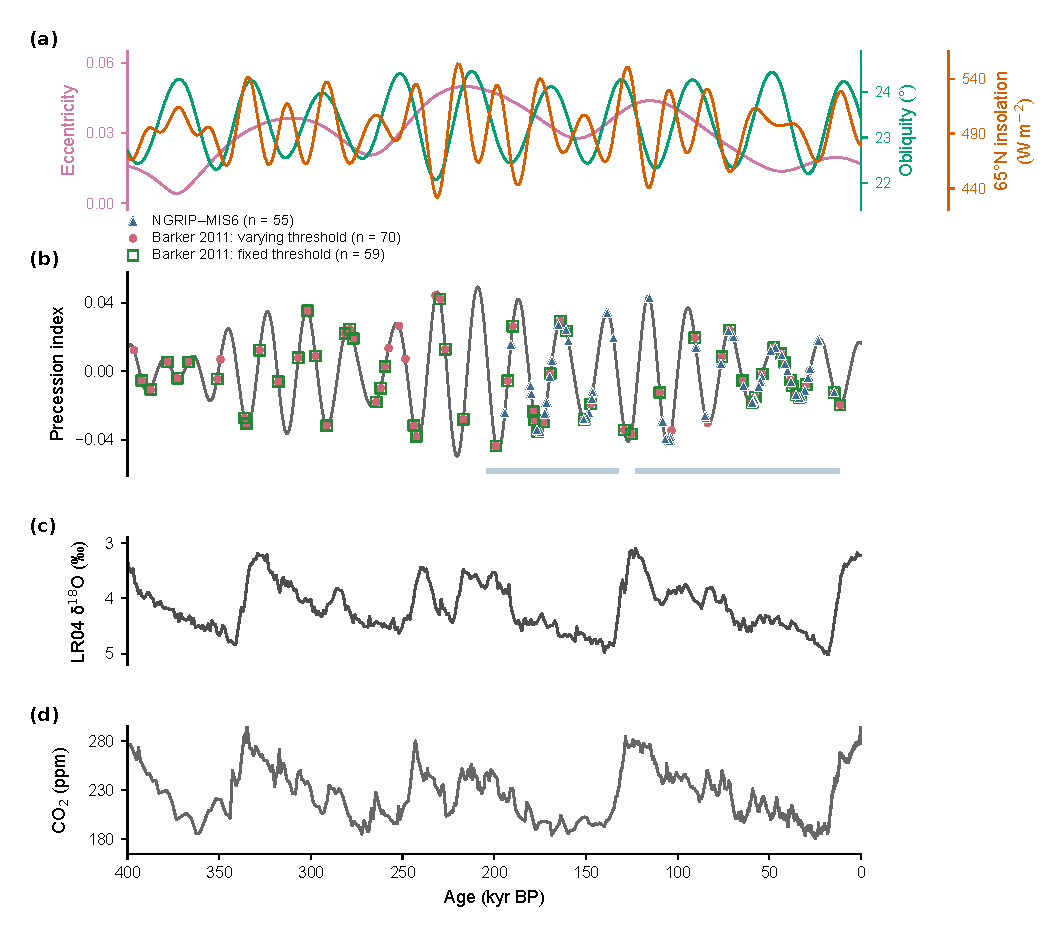
\includegraphics[width=\linewidth,height=0.68\textheight,keepaspectratio]{figures/Fig01.pdf}
\caption{Event inventories and environmental context. (a) Eccentricity, obliquity, and daily mean summer-solstice insolation at $65^\circ$N from the orbital solution of \citet{laskar2004long} (La2004); axes match curve colors. (b) Precession index with NGRIP--MIS6 events (blue triangles; 55), Barker varying-threshold events (rose circles; 70), and the fixed-threshold subset (open green squares; 59). Blue strips mark the observation intervals of NGRIP--MIS6 events; Barker spans 0--400 kyr BP. (c) LR04 benthic $\delta^{18}$O \citep{lisiecki2005pliocene}. (d) Antarctic composite Atmospheric CO$_2$ data \citep{bereiter2015revision}. Event sources are \citet{rasmussen2014stratigraphic,fohlmeister2023role,held2024dansgaard,barker2011800}.}
\label{fig:data_framework}
\end{figure}

We represent background climate using LR04 benthic $\delta^{18}$O and the Antarctic atmospheric CO$_2$ composite \citep{lisiecki2005pliocene,bereiter2015revision}. LR04 reflects both ice volume and deep-water temperature. Orbital inputs follow the solution of \citet{laskar2004long} (La2004). Phase is interpolated between alternating precession-index extrema: minima define $0^\circ$, maxima $180^\circ$, and phase increases toward older ages.

We model warming onsets as events in continuous time, allowing their occurrence rate to change with background climate, recent events, and precession phase \citep{truccolo2005point,kass2014analysis}. The conditional intensity $\lambda_r(t)$ is the instantaneous warming rate in events per kyr for record segment $r$: over a short interval $dt$, the probability of a warming is approximately $\lambda_r(t)dt$, given the preceding events. To make time advance toward the present, we convert BP age $a$ to elapsed time $t=a_{r0}-a$, where $a_{r0}$ is the age of the segment's oldest event. This event sets $t=0$ and initializes the history. The full model is
\begin{equation}
\log\lambda_r(t)=\beta_0+\beta_H H_r(t)+\beta_L L_r(t)+\beta_C C_r(t)+\beta_S S_r
+\beta_s\sin\phi_r(t)+\beta_c\cos\phi_r(t),\label{eq:rate}
\end{equation}
where $L_r$ and $C_r$ are scaled LR04 and CO$_2$ values. Each variable is centered on its mean over the fitted intervals and divided by its maximum--minimum range across those intervals. For NGRIP--MIS6, this mean combines the time averages within the NGRIP and MIS~6 segments, weighted by the lengths of their respective fitted intervals; the gap between the records is excluded. Both segments share the resulting mean and range. Barker uses its own fitted interval. These scaling means and ranges remain fixed in subsequent simulations and sensitivity tests for that catalogue. $S_r$ is zero for NGRIP and one for MIS~6, allowing their baseline rates to differ. This term is omitted for the single Barker record. The sine and cosine terms allow the rate to vary smoothly over the precession cycle. Modeling the logarithm keeps the rate positive.

The history term gives greater weight to more recent events:
\begin{equation}
H_r(t)=\sum_{j:0\leq t_{rj}<t}\exp[-(t-t_{rj})/\tau].
\end{equation}
Each earlier event contributes one immediately after it occurs, and its contribution falls to $1/e$ after $\tau=1.5$ kyr. Only events in the same segment contribute, including the oldest event used for initialization. We set the contribution from unobserved events before that starting point to zero. Constraining $\beta_H\leq0$ allows recent events to suppress the rate, with this influence weakening as time passes. This choice is motivated by the time needed for sea ice and ocean circulation to evolve through an interstadial and re-establish conditions for another abrupt warming \citep{dokken2013dansgaard,vettoretti2022atmospheric}. The decay time and initialization are tested in sensitivity analyses (Text~S5).

We estimate coefficients by maximizing the conditional log likelihood \citep{daley2003introduction},
\begin{equation}
\ell=\sum_r\left[\sum_{i=1}^{N_r}\log\lambda_r(t_{ri})-\int_0^{T_r}\lambda_r(t)\,dt\right],\label{eq:likelihood}
\end{equation}
where $N_r$ counts fitted events after the oldest event and $T_r$ is the time from that oldest event to the younger observation boundary. The first term favors high modeled rates at observed warmings. The second penalizes high rates across the entire fitted interval, including periods with no events. History at an event uses only preceding events, so an event cannot help predict itself. Climate values are interpolated at the event times and at the points used for numerical integration (Text~S2). The model describes warming occurrence over the whole observation interval, including both cold and warm periods.

To test whether precession adds information, we compare this full model with a background model (BG) containing the same climate, history, and segment terms but no phase terms. All coefficients are fitted separately in each model. We summarize the improvement using the log-likelihood gain per event, $G$, and the likelihood-ratio statistic, $LR$:
\begin{equation}
G=\frac{\ell_{\mathrm{full}}-\ell_{\mathrm{BG}}}{N\ln2},\qquad
LR=2(\ell_{\mathrm{full}}-\ell_{\mathrm{BG}}),\label{eq:gain}
\end{equation}
where $N=\sum_r N_r$ is the number of fitted events. $G$ measures the average improvement in fit in bits/event; it describes the observed sequence rather than prediction of new records. We also report the phase with the highest fitted rate and the ratio between maximum and minimum rates over a phase cycle (Figure~\ref{fig:phase_comparison}), at fixed climate and history (Text~S2). An unadjusted Rayleigh test of event-phase concentration is reported separately in Text~S2.

To compare the conditional contributions of precession and background climate, we also fit a model that retains precession but omits LR04 and CO$_2$. We compare the full model with each reduced model, expressing both likelihood gains in bits per fitted event (Text~S7; Figure~S6). Each comparison adds two coefficients and refits all remaining coefficients, while keeping event history, segment terms, and observation intervals unchanged. These gains measure the contribution of each predictor block after accounting for the other, and they do not partition the total information into additive shares.

Unless stated otherwise, $p$ values for likelihood-ratio comparisons use the asymptotic $\chi^2$ distribution, with degrees of freedom equal to the number of added coefficients. These nominal tests account for the improvement expected from adding parameters, but the approximation may be inaccurate for our small event catalogues with history dependence and parameter constraints. We therefore check the main phase results using a parametric bootstrap \citep{davison1997bootstrap}. For the primary catalogue and each Barker event definition, we simulate 9,999 event sequences from its fitted BG model, which has no phase dependence, and refit both BG and full. Simulations retain each segment's oldest event and younger boundary, allow event totals to vary, and update history whenever an event occurs. Climate covariates are interpolated at the simulated event times using the same climate records and fixed scaling means and ranges. If $b$ simulated $LR$ values equal or exceed the observed value, $p_{\rm boot}=(b+1)/10{,}000$ (Text~S2). This checks sensitivity to the reference distribution under the fitted null model; it does not include age uncertainty.

Separate simulations test whether event history improves the fit beyond climate and phase. We also check how well the full model reproduces event spacing, using the 5,000 nominal-age full-model simulations and refits per catalogue described in Text~S4. After adjusting intervals for changes in the fitted rate, we compare their distribution and the association between neighboring intervals with those in the simulated sequences (Text~S2).

To assess the sensitivity of the phase association to chronology uncertainties, we generate 10,000 Monte Carlo (MC) event sequence realizations, preserving event identities and order. Record-specific perturbations represent correlated chronology shifts and, for NGRIP and the speleothems, uncertainty in locating event onsets (Text~S3; Figures~S3--S5). The modeled NGRIP extension uses an assumed uncertainty envelope because published errors are unquantified \citep{corrick2020synchronous}. For each realization within the observation windows, we refit both models, rebuilding event history and the fitted interval from each segment's realized oldest event while retaining nominal climate scaling (Text~S3).

We also ask how precisely each main catalogue determines the preferred phase and the strength of rate modulation. Perturbing the ages of the observed events captures age uncertainty, but another event sequence generated under the same climate conditions could yield a different fitted effect due to the stochastic nature of climate processes. To assess this sampling uncertainty, we generate and refit new sequences from the fitted full model, retaining its phase dependence (Text~S4). We compare chronology uncertainty, sampling at fixed chronology, and sampling combined with chronology uncertainty (Figure~\ref{fig:effect_precision} for NGRIP--MIS6 and Figure~S7 for Barker). We obtain preferred-phase and rate-ratio bounds from joint regions for the two phase coefficients. Sampling simulations give approximate confidence limits; chronology and combined ensembles give sensitivity ranges (Text~S4).

We test the phase result against alternative history decay, initial history, climate-response shapes, and separate phase responses for the two primary segments (Text~S5). Event-catalogue checks compare Barker event definitions, apply the model separately to NGRIP warming and cooling onsets, and randomly delete events to assess additional inventory loss (Text~S6).

Finally, we compare precession phase with eccentricity, obliquity, and summer-solstice insolation at $65^\circ$N (Text~S7; Figure~S10). For each variable, we test its contribution before and after including precession phase, and the contribution of precession phase after including that variable. We adjust the nominal $p$ values for these nine additional comparisons within each catalogue using Holm's procedure \citep{holm1979simple}.

\section{Results}
Precession phase improves the primary event-rate fit by $G=0.2482$ bits per fitted event ($LR=18.238$), with nominal $p=0.000110$ and bootstrap $p=0.0003$ (Figure~\ref{fig:phase_comparison}). The association therefore persists under bootstrap calibration. At fixed background climate and history, the fitted rate is highest at $328.1^\circ$, near the precession-index minimum, and is 7.18 times its minimum over the phase cycle. The full model produces a peak in expected counts near the observed concentration, whereas the BG model gives a nearly flat phase distribution (Figure~\ref{fig:phase_comparison}a).

Barker variable-threshold events favor a similar phase, with $G=0.1106$ bits per fitted event, nominal $p=0.00504$, bootstrap $p=0.0077$, a maximum at $334.2^\circ$, and a smaller rate ratio of 3.32 (Figure~\ref{fig:phase_comparison}d). Fixed-threshold events give $G=0.1067$, nominal $p=0.0137$, bootstrap $p=0.0172$, a maximum at $347.1^\circ$, and a rate ratio of 3.19 (Figure~\ref{fig:phase_comparison}c,d). Both definitions receive their own bootstrap calibration at unperturbed ages.

\begin{figure}[p]
\centering
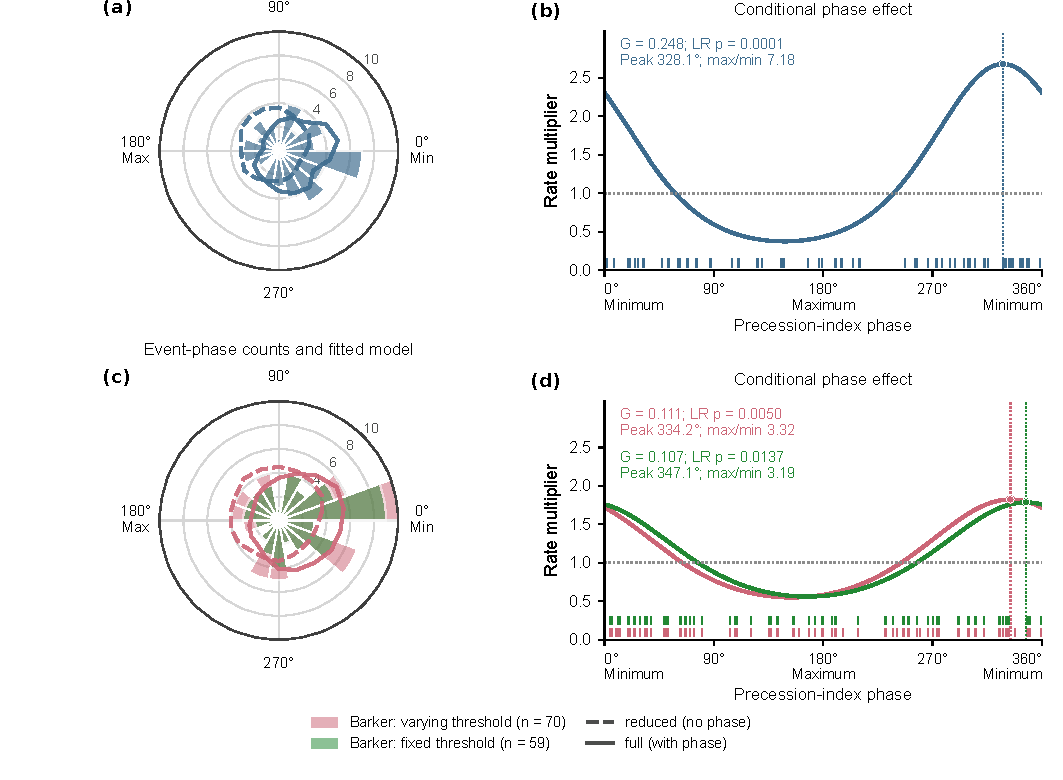
\includegraphics[width=\linewidth,height=0.775\textheight,keepaspectratio]{figures/Fig02.pdf}
\captionsetup{font=footnotesize}
\caption{Event phases and the fitted phase effect. Blue, rose, and green identify NGRIP--MIS6, Barker varying threshold, and Barker fixed threshold, respectively \citep{rasmussen2014stratigraphic,fohlmeister2023role,held2024dansgaard,barker2011800}. (a,c) Observed counts in $20^\circ$ phase sectors (bars), with expected counts from the BG model without phase (dashed) and the full model (solid) for the NGRIP-MIS6 and Barker varying-threshold catalogues. (b,d) The factor $\exp(\beta_s\sin\phi+\beta_c\cos\phi)$ by which phase multiplies the full model's rate at fixed climate and history; dots mark its maximum and bottom ticks mark observed event phases. A factor of one means that the phase terms make no contribution at that angle. Annotations give $G$, the full-minus-BG log-likelihood gain in bits per fitted event. The corresponding bootstrap $p$ is calibrated using likelihood ratios from 9,999 simulations under each catalogue's fitted BG model. Preferred phase and maximum/minimum rate ratio are estimated from the fitted full model. Minimum/Maximum axis labels refer to the precession index. Histograms in a,c show all 55/70/59 events, while model fits use 53/69/58 events after excluding each starting event. Ages are unperturbed; age uncertainty is assessed separately.}
\label{fig:phase_comparison}
\end{figure}

The phase association generally persists when chronology uncertainties are considered (Text~S3). Nominal $p<0.05$ in 99.79\% of valid NGRIP--MIS6 fits and 99.48\% of Barker fits; the complete age-ensemble results, including the ranges of $G$, are reported in Text~S3. 

The full-model simulations show that a statistically supported phase association can still have an imprecisely estimated strength (Figure~\ref{fig:effect_precision}). For the NGRIP-MIS6, the chronology-only uncertainty gives preferred-phase bounds of $309.1^\circ$--$351.3^\circ$ and a rate-ratio range of 3.74--14.14. The sampling (or realization) uncertainty gives $287.8^\circ$--$10.2^\circ$ and 1.73--29.88 (angles above $360^\circ$ continue into the next cycle). Combining chronology uncertainty and realization uncertainty gives $287.1^\circ$--$15.2^\circ$ and 1.69--30.77. These values are calculated from the 95\% range of the precession phase coefficients, corresponding to the elliptical region in coefficient space that contains 95\% of the data points (Figure~\ref{fig:effect_precision}, Text~S4). The preferred part of the cycle remains broadly localized, but the modulation strength is imprecise in both the NGRIP-MIS6 and Barker catalogues (Figure~\ref{fig:effect_precision}; Figure~S7).

\begin{figure}[p]
\centering
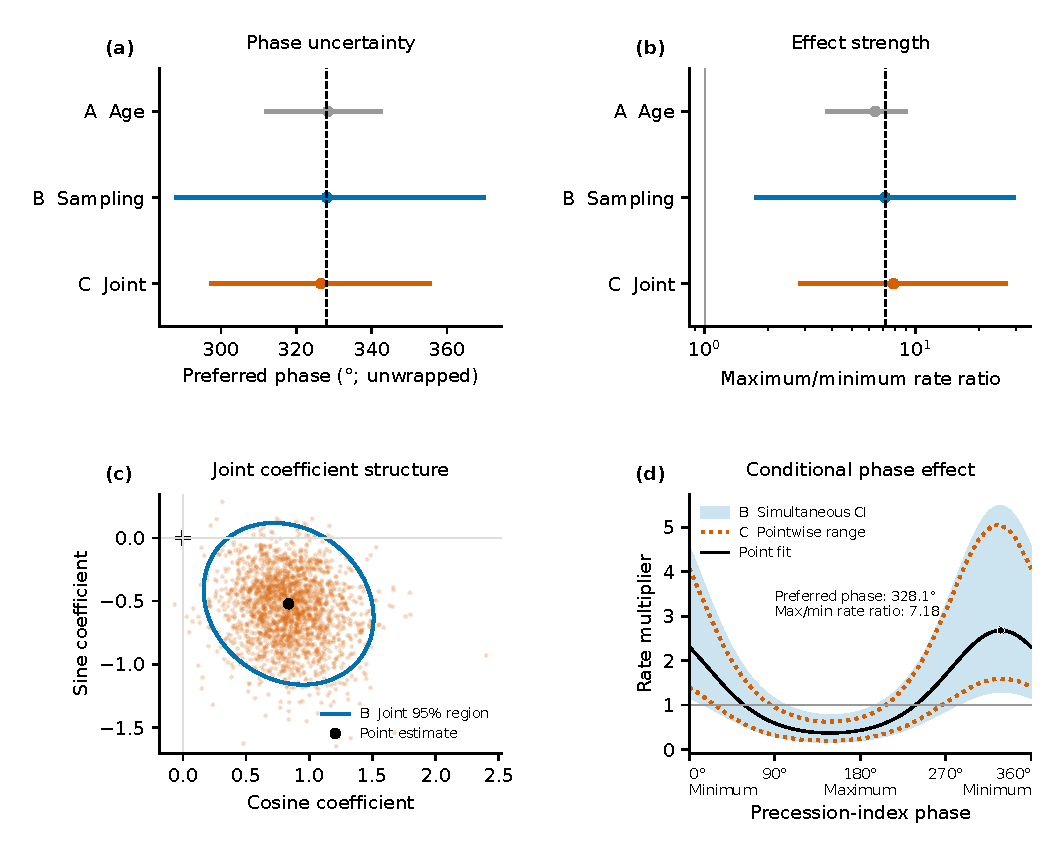
\includegraphics[width=\linewidth,height=0.68\textheight,keepaspectratio]{figures/Fig03.pdf}
\caption{Uncertainty in the primary phase effect (Texts~S3 and S4). Chronology (gray dotted), sampling (blue solid), and sampling + chronology (orange dashed) use the same coefficient-ellipse construction. (a,b) Preferred-phase and maximum/minimum rate-ratio bounds projected from the 95\% regions in (c); dots and dashed vertical lines mark nominal estimates, and phase angles continue across $360^\circ$. (c) Coefficient regions, nominal estimate (black dot), and no phase effect (cross). (d) Rate multiplier envelope of the region shown in c. The black curve, black dots, blue lines, and orange dashed lines mark the rate multiplier of the nominal age and its 95\% regions when considering chronology uncertainty, sampling uncertainty, and sampling + chronology uncertainty, respectively. Unity means no phase contribution. }
\label{fig:effect_precision}
\end{figure}

The primary association also persists when model assumptions are varied (Text~S5). Changing the history decay time from 1 to 5 kyr gives $G$ 0.243--0.252 and phase maxima $318.2^\circ$--$330.3^\circ$, with the same fitted events and time intervals. Allowing a contribution from events before each segment's starting point has little effect ($G$ 0.248--0.250; Figure~S8). Allowing non-linear rather than linear responses of backgroud climate variables gives $G$ 0.239--0.252. Replacing the exponential history with the count of events in the preceding 1.5 kyr gives $G$ 0.219 and a $332.4^\circ$ maximum; using time since the preceding event gives $G$ 0.202--0.209 (Figure~S9). Allowing NGRIP and MIS~6 to have different phase responses does not clearly improve the fit (nominal $p=0.810$). Separate simulation tests support including event history (Text~S2).

At nominal ages, neither main catalogue shows a clear mismatch between observed and modeled event spacing. After accounting for changes in the fitted rate, the observed distribution of interval lengths and the association between neighboring intervals show no unusual departures compared with simulated and refitted sequences (Text~S2).

Summer-solstice insolation and precession phase explain some of the same variation in event occurrence (Figure~S10; Text~S7). Adding insolation to BG gives $G$ 0.184 for the NGRIP-MIS6 and 0.063 for Barker. Once precession phase is included, the additional insolation gains fall to 0.049 and 0.002. Likewise, precession phase contributes less after insolation is included: $G$ is 0.113 and 0.050, compared with 0.248 and 0.111 when precession phase is added to BG alone. Neither precession phase test after insolation passes the Holm correction of nominal $p$ values (adjusted $p=0.093$ and 0.560). Eccentricity and obliquity add little after precession phase, while precession phase remains associated with occurrence of DO events after allowing for obliquity (Holm-adjusted nominal $p=0.000394$ and 0.0368).

An exploratory analysis of NGRIP cooling onsets gives a preferred phase close to that of warming onsets in the same record (Text~S6). After accounting for LR04, CO$_2$ and recent cooling events, adding precession phase improves the fit by $G=0.136$ bits/event, with a rate maximum at $340.1^\circ$, compared with $327.1^\circ$ for the separate NGRIP warming fit. Evidence for the cooling association is weaker: nominal $p=0.0408$, but bootstrap $p=0.0721$. Nominal $p<0.05$ in 5,433 of 9,263 valid age realizations (58.7\%). Thus, cooling onsets favor a similar phase sector at nominal ages, but the association is less robust to bootstrap calibration and age uncertainty, which may partly reflect the small event count.

\section{Discussion}

Our results identify a preferred orbital configuration for abrupt warming after accounting for the modeled effects of background climate and recent-event history. The fitted onset rate peaks near the precession-index minimum in both the NGRIP-MIS6 and the Barker catalogue comparison, although the strength of this modulation remains imprecisely estimated. The magnitude of the conditional gains places the phase association in a broader context: precession contributes fit information comparable to that provided by LR04 and CO$_2$ after accounting for phase (Figure~S6), with more frequent DO events preferring precession minima.This extends earlier statistical comparisons in which the relative support for ice-volume and insolation forcing depended on the assumed dynamics \citep{mitsui2017influence}. Taken together, the preferred phase and comparable conditional gains support an important role for orbital configuration in regulating DO recurrence within glacial climates.

The overlapping contributions of precession phase and summer-solstice insolation suggest that seasonal insolation links orbital configuration to DO recurrence (Figure~S10). Changes in seasonal forcing could affect both whether repeated transitions are sustained and how rapidly they recur (Figure~\ref{fig:orbital_mechanism}). Under intermediate glacial conditions, reduced precession and enhanced boreal seasonality intensified the tropical Atlantic warm pool and reduced atmospheric moisture export, freshening waters whose northward transport initially weakened deep-water formation. Then under constant orbital forcing, coupled changes in subsurface heat, northward salt transport, and sea ice sustain repeated transitions between weak and strong AMOC states \citep{zhang2021direct}. Within an oscillatory regime, stronger boreal seasonality can also shorten stadials and interstadials through changes in sea-ice thickness and ocean heat loss, lead to more frequent DO events \citep{kuniyoshi2022effect}. Changing the conditions required for individual transitions offers one way to produce these responses. For example, \citet{fohlmeister2023role} proposed that stronger summer insolation amplifies initial sea-ice retreat through the ice--albedo feedback, lowering the subsurface-temperature threshold for entering an interstadial. If subsurface heat accumulates at a similar rate, a lower threshold can shorten the cold interval; if the threshold was previously unreachable, lowering it may enable a transition that would otherwise not occur. Changes in transition thresholds and recurrence times are therefore closely connected. These mechanisms provide plausible explanations for the higher warming rate near precession minima, through changes in the conditions that sustain repeated transitions, the time needed to complete a cold--warm cycle, or both (Figure~\ref{fig:orbital_mechanism}).

Together with previous findings, our results provide a calibration target for climate model simulations of DO events. In the experiments of \citet{snoll2025competing}, changes in sea-ice freshwater release and thermal insulation altered both the duration of warm phases and whether the circulation returned to a cold state. Some orbital configurations shortened warm phases, whereas others favored faster, smaller-amplitude fluctuations within relatively warm conditions. These different responses highlight the value of evaluating event occurrence and variability amplitude together. Our finding that warming onsets favor precession minima adds an event-based constraint to earlier evidence for orbital modulation of MCV amplitude \citep{sun2021persistent,hodell20231,thirumalai2020methane}. Together, these observations provide two complementary targets for climate simulations: the orbital phase at which abrupt warmings occur most frequently, and the orbital modulation of the amplitude of millennial-scale variability. Model–data comparisons should assess these features under comparable background conditions, examining warming-onset rates alongside transition amplitudes, and the amplitude envelope of filtered climate variability. 

Viewed in the broader context, the preferred precession phase also provides an observational constraint on how glacial boundary conditions and internal climate feedbacks combine to produce DO activity. Ice-sheet geometry can alter AMOC stability through changes in winds and ocean--sea-ice transport \citep{zhang2014abrupt}, while atmospheric CO$_2$ influences whether the climate remains relatively stable or develops spontaneous oscillations \citep{vettoretti2022atmospheric,zhang2017abrupt}. Across three climate models, North Atlantic sea-ice coverage provides a common indicator of conditions supporting DO-like oscillations, despite differences in their amplitude, duration, and shape \citep{malmierca2024impact}. Even at similar ice volume and atmospheric CO$_2$, differences in seasonal insolation can alter sea-ice growth and melt, ocean heat loss, and the approach to convective instability. Our phase preference suggests that these seasonally sensitive processes may help explain differences in DO recurrence that are not captured by the background indicators alone.




\begin{figure}[p]
\centering
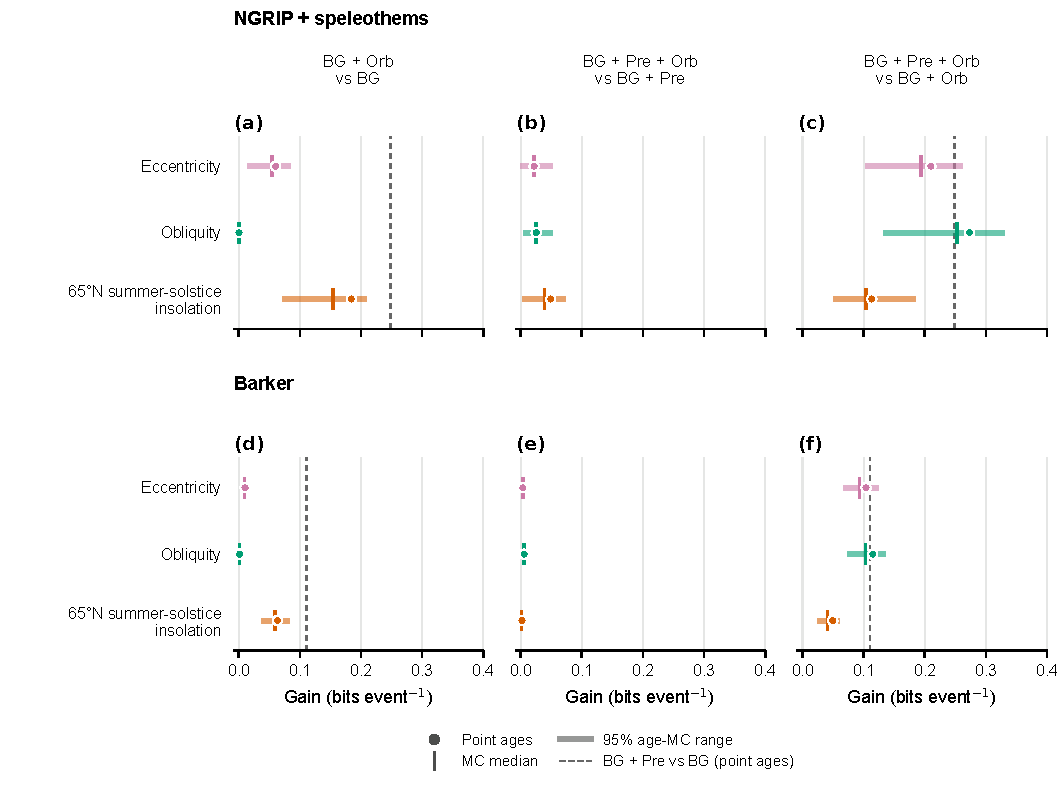
\includegraphics[width=\linewidth]{figures/Fig04.pdf}
\caption{Proposed pathways linking low precession and stronger Northern Hemisphere (NH) seasonality to DO recurrence. (a) A warmer Atlantic warm pool reduces moisture export to the Pacific; fresher water transported north increases stratification and initially weakens the AMOC, after which internal feedbacks can sustain oscillations \citep{zhang2021direct}. (b) Thinner sea ice can favor earlier warming, while greater winter heat loss from open water can shorten the warm state \citep{kuniyoshi2022effect}. Stronger summer insolation may amplify initial sea-ice retreat through the ice--albedo feedback, lowering the subsurface-temperature threshold for interstadial onset (dashed arrow) \citep{fohlmeister2023role}. The corresponding blue downward arrow marks the cooling during DO cycles. Cyan ice sheets and white sea ice depict a schematic stadial background, with illustrative ice sheet margin inspired by \citet{zhang2017abrupt}.  
        }
\label{fig:orbital_mechanism}
\end{figure}



The small additional contribution from obliquity does not exclude its influence on DO activity. Our comparison asks whether obliquity explains event occurrence beyond LR04, CO$_2$, recent events and precession phase. It therefore measures information not already represented by these predictors, rather than the total climatic influence of obliquity. Ice-volume records themselves contain information about orbital forcing \citep{lisiecki2005pliocene}, so an obliquity influence expressed through changes in background climate could be partly absorbed by our climate terms. A single linear obliquity term may also miss a response that depends on climate state. The weak additional association therefore does not exclude the physical influences of obliquity on MCV suggested by climate-model experiments \citep{zhang2021direct,snoll2025competing}.

Several limitations affect how firmly these mechanisms can be evaluated. Regional speleothems and the synthetic Barker reconstruction may capture different subsets of abrupt changes. Random deletion tests generally preserve the preferred phase, but do not test omissions that depend on orbital phase (Text~S6). The absence of an obvious mismatch in event spacing does not mean that the model captures all climatic controls on DO recurrence (Text~S2). The limited event count also leaves the strength of phase modulation poorly constrained, even though the bootstrap tests support a phase association (Figure~\ref{fig:effect_precision}; Figure~S7).

Background climate can also change which orbital configurations favor DO activity. In the experiments of \citet{zhang2021direct}, orbital changes produced no AMOC mode switches under the tested peak-glacial and interglacial conditions. Statistical analysis of Antarctic records shows that the rate of Antarctic warming during Greenland stadials declined as the background climate cooled through MIS~3, illustrating changes in the expression of MCV within intermediate glacial conditions \citep{zheng2021different}. This raises a more specific question for our analysis: within background climate conditions favorable to DO activity, does background climate alter the strength or preferred phase of the precession response? Our catalogues constrain a common phase response across the fitted intervals, rather than mapping how it changes within intermediate glacial conditions. Resolving such changes will require more extensive, well-dated event sequences spanning different combinations of background climate and orbital phase, together with complementary indicators of background climate beyond LR04 and atmospheric CO$_2$.


\section{Conclusions}

Using a continuous-time event-rate model, we identify a preferred precession phase for abrupt warming after accounting for LR04, atmospheric CO$_2$, and recent-event history. The Greenland--speleothem catalogue and the synthetic Greenland comparison both favor phases near the precession-index minimum. Bootstrap calibration and sensitivity tests support this association, while event-sequence simulations show that its strength remains imprecisely estimated due to the chronology uncertainties and limited event number. Within the specified model, the conditional fit contribution of precession is comparable to that of the background-climate indicators, emphasizing the information that orbital configuration adds to explanations of DO recurrence. 

The overlapping contributions of precession and summer insolation link this phase preference to seasonal forcing. Together with climate-model evidence, the results are consistent with orbital changes favoring conditions for repeated ocean--sea-ice transitions, shortening cold--warm cycles, or both. Distinguishing these responses requires more extensive, well-dated records of both warming and cooling onsets, together with the durations and amplitudes of the associated climate states. Targeted simulations should vary orbital configuration across comparable glacial backgrounds and test whether their mechanisms reproduce these features jointly. Such comparisons would clarify how seasonal forcing alters internal climate feedbacks and whether the preferred orbital configuration changes within intermediate glacial conditions.


\section*{Abbreviations}

This list covers the main text, Supporting Information, and figure labels. Time units are yr (years), kyr or ka (thousand years), and Myr (million years); ppm denotes parts per million.

\begin{description}
\setlength{\itemsep}{0pt}
\setlength{\parsep}{0pt}
\item[AIC] Akaike information criterion
\item[AMOC] Atlantic Meridional Overturning Circulation
\item[BG] background model, including climate and event-history terms
\item[BP] before present, with present defined as 1950 Common Era
\item[DO] Dansgaard--Oeschger
\item[GI] Greenland Interstadial
\item[GICC05] Greenland Ice-Core Chronology 2005
\item[GICC05modelext] flow-model extension of GICC05
\item[GS] Greenland Stadial
\item[LR] likelihood ratio
\item[LR04] benthic $\delta^{18}$O stack of Lisiecki and Raymo (2005)
\item[MC] Monte Carlo
\item[MCE] maximum counting error
\item[MCV] millennial-scale climate variability
\item[MF] Melchsee--Frutt
\item[MIS] Marine Isotope Stage
\item[NGRIP] North Greenland Ice Core Project
\item[NH] Northern Hemisphere
\item[Orb] scalar orbital predictor used in model comparisons
\item[Pre] precession-phase sine and cosine terms
\end{description}

\section*{Open Research}
The Greenland event inventory follows \citet{rasmussen2014stratigraphic}; the Greenland Ice-Core Chronology 2005 (GICC05) data are archived by \citet{rasmussen2022gicc05}. MF and Sofular source data are archived by \citet{fohlmeister2023mfData,held2024sofularData}. The synthetic Greenland event catalogue and its chronology controls are supplied by \citet{barker2011800}. Background and orbital inputs follow \citet{lisiecki2005pliocene,bereiter2015revision,laskar2004long}. The analysis code for this study is available at \url{https://github.com/Peisong-Zheng/MCV_ORB}.

\section*{Acknowledgements and author statements}
\emph{This work was supported by the UKRI Centre for Doctoral Training in Application of Artificial Intelligence to the study of Environmental Risks (reference EP/S022961/1).}

\bibliographystyle{agu}
\bibliography{reference}
\end{document}
